\input{../YKY-preamble.tex}

\usepackage{color}
\usepackage{mathtools}
\usepackage{hyperref}

% \usepackage[backend=biber,style=numeric]{biblatex}
% \bibliography{../AGI-book}
% \renewcommand*{\bibfont}{\footnotesize}

\usepackage{graphicx} % Allows including images
\usepackage{tikz-cd}
\usepackage{tikz}
\usetikzlibrary{shapes}
\usepackage[export]{adjustbox}% http://ctan.org/pkg/adjustbox
\usepackage{bm}
\usepackage{verbatim} % for comments
\usepackage[most]{tcolorbox}
% \usepackage{newtxtext,newtxmath}	% Times New Roman font

\setcounter{secnumdepth}{1}		% no sub-section numbers
% \numberwithin{equation}{subsection}

\newcommand{\underdash}[1]{%
	\tikz[baseline=(toUnderline.base)]{
		\node[inner sep=1pt,outer sep=10pt] (toUnderline) {#1};
		\draw[dashed] ([yshift=-0pt]toUnderline.south west) -- ([yshift=-0pt]toUnderline.south east);
	}%
}%

\newcommand{\bO}[0]{$\pmb{\bm{\Circle}}$}
\newcommand{\bX}[0]{$\pmb{\bm{\times}}$}

\DeclareSymbolFont{symbolsC}{U}{txsyc}{m}{n}
\DeclareMathSymbol{\strictif}{\mathrel}{symbolsC}{74}

\newcommand{\highlight}[1]{\colorbox{pink}{$\displaystyle #1$}}

\newcommand{\emp}[1]{{\color{violet}\textbf{#1}}}
\newcommand*\confoundFace{$\vcenter{\hbox{\includegraphics[scale=0.2]{../2020/../confounded-face.jpg}}}$}
\newcommand{\underconst}{\includegraphics[scale=0.5]{../2020/UnderConst.png}}
\newcommand{\witness}{\scalebox{0.6}{$\blacksquare$}}
% \newcommand{\Heytingarrow}{\mathrel{-}\mathrel{\triangleright}}
\providecommand\Heytingarrow{\relbar\joinrel\mathrel{\vcenter{\hbox{\scalebox{0.75}{$\rhd$}}}}}

\newcommand{\bbb}[1]{\tcbox[size=small, colback=yellow!10!white, box align=base, nobeforeafter]{#1}} 

\begin{document}

\title{\bfseries\color{blue}{\Huge AGI for dummies}}
\author{YKY} % Your name
%\institute[] % Your institution as it will appear on the bottom of every slide, may be shorthand to save space
%{
%Independent researcher, Hong Kong \\ % Your institution for the title page
%\medskip
%\textit{generic.intelligence@gmail.com} % Your email address
%}
\date{\today} % Date, can be changed to a custom date

\maketitle

% \vspace*{0.5cm}
% 多谢 支持 \smiley

% \setcounter{section}{-1}
\subsection{Language models and how they are trained}

As of 2022, the most ``intelligent'' AI systems are \textbf{language models} such as BERT, GPT-3, .... and their variants.

These systems are trained to understand natural language, using a revolutionary technique by \textbf{masking out} words in a text corpus and asking the AI to \textbf{predict} them.  For example:
\begin{eqnarray}
\nonumber
\bbb{All} \; \bbb{work} \; \bbb{and} \; \bbb{no} \; \bbb{play} & \bbb{makes} \; \bbb{Jack} \; \bbb{a} \; \bbb{dull} \; \bbb{boy} \\
\Downarrow & \\
\bbb{All} \; \bbb{work} \; \bbb{and} \; \bbb{no} \; \bbb{\color{red}???} & \bbb{makes} \; \bbb{Jack} \; \bbb{a} \; \bbb{dull} \; \bbb{boy} 
\nonumber
\end{eqnarray}
When a neural network is \textbf{forced} to make such predictions, it will gradually start to acquire knowledge similar to human's.  This knowledge is stored in the (massive number of) \textbf{weights} in the neural network.

Using the masked-word trick, there is no longer the need to prepare \textbf{annotated} data to train the AI, solving one of the biggest bottlenecks in AI development.

\subsection{Transformers -- the most advanced AI component}

The above language models are based on a key component known as \textbf{Transformers}, invented by a research team in Google:
\begin{equation}
\vcenter{\hbox{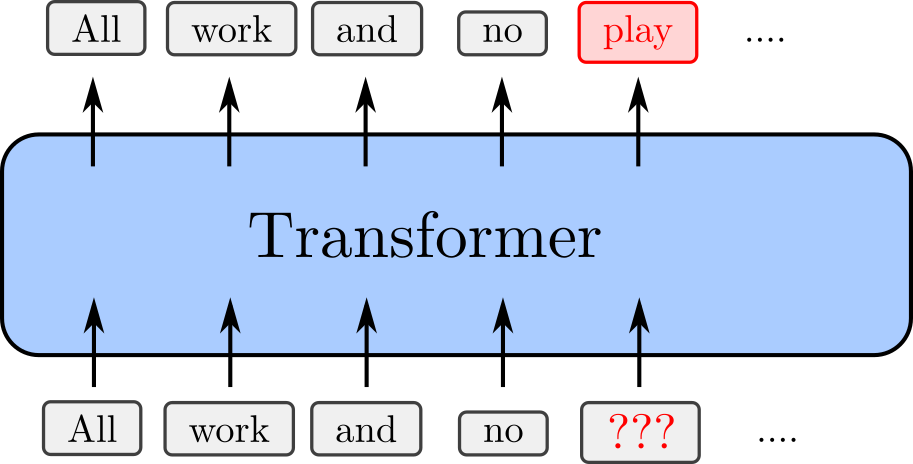
\includegraphics[scale=1]{Transformer_next-word-predict.png}}}
\end{equation}

In principle, we only need a ``fully-connected'' neural network and train it to predict the masked words.  But such a network without \textbf{additional structure} is too inefficient to learn the desired knowledge.  One of the key ideas in machine learning is to give a machine some ``\textbf{bias}'' to make it learn faster.  An example of bias is to ``cut'' some connections in a fully-connected neural network, so that it looks like partitioned into blocks.

The Transformer has an internal structure known as the \textbf{Attention} mechanism.  It looks like this:
\begin{equation}
\vcenter{\hbox{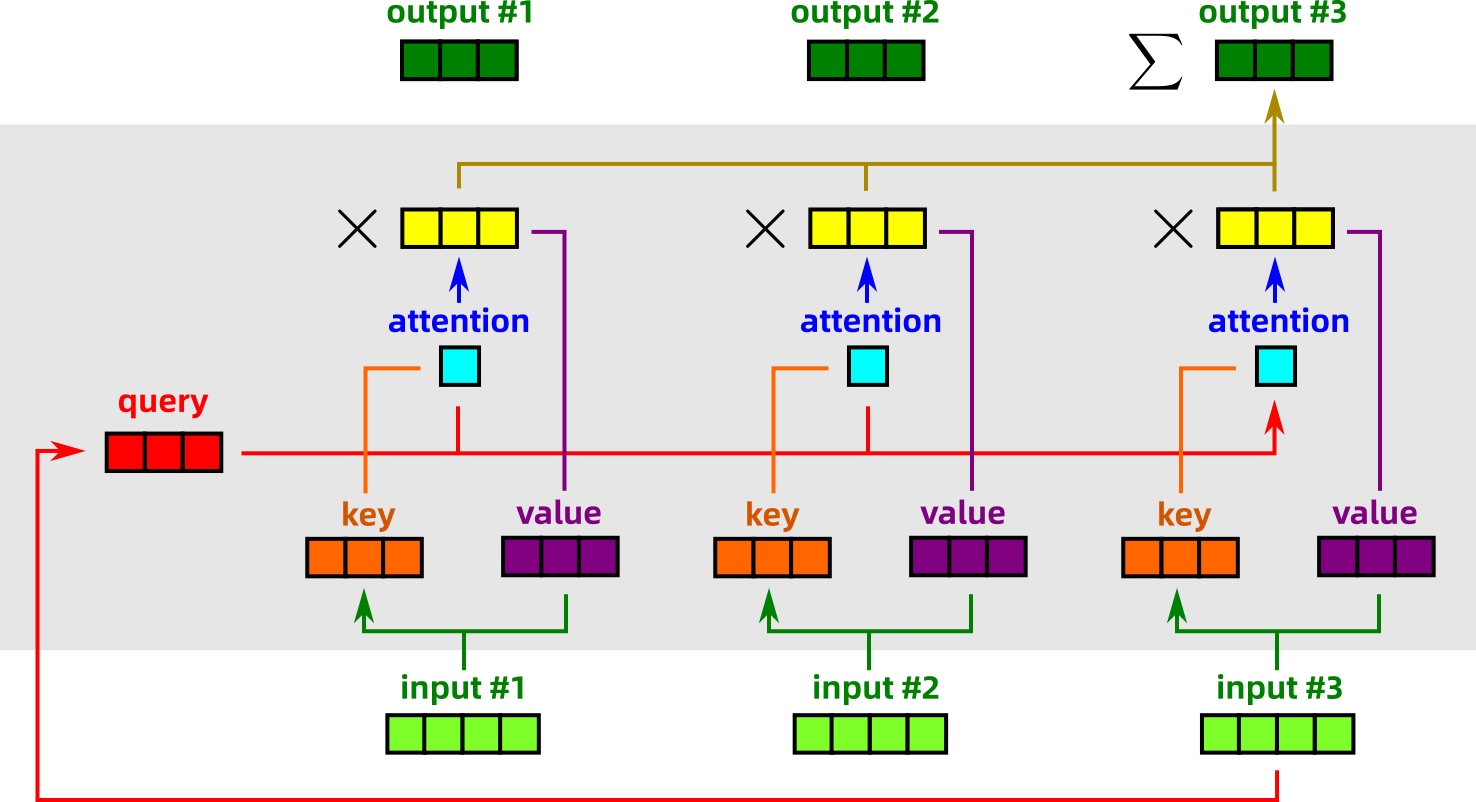
\includegraphics[scale=0.9]{self-attention-2.png}}}
\end{equation}

This is not widely accepted, but my hypothesis is that \uline{the Transformer performs logic reasoning}.

\subsection{Logic as a form of rewriting}

The following are examples of \textbf{logic rules}:

``All humans are mortal'':
\begin{equation}
{\color{red}\forall x.} \; \mbox{human}({\color{red}x}) \Rightarrow \mbox{mortal}({\color{red}x}) \\
\end{equation}
``The father's father is the grand-father'':
\begin{equation}
{\color{red}\forall x, y, z.} \; \mbox{father}({\color{red}x,y}) \wedge \mbox{father}({\color{red}y,z}) \Rightarrow \mbox{grand-father}({\color{red}x,z}) 
\end{equation}

The symbol $\forall$ means ``for all'', $\wedge$ means ``and'', $\Rightarrow$ means ``imply''.

In order for the logic formulas to work, variables such as $x, y, z$ need to be \textbf{copied} from the left-hand-side \textbf{premise} to the right-hand-side \textbf{conclusion}.  For example:
\vspace{-10pt}
\begin{eqnarray}
\mbox{human({\color{red}Socrates})} \tikzmark{s1} & \Rightarrow & \mbox{mortal({\color{red}Socrates})} \tikzmark{s2} \nonumber \\[10pt]
\mbox{human({\color{red}Plato})} \tikzmark{p1} & \Rightarrow & \mbox{mortal({\color{red}Plato})} \tikzmark{p2}
\begin{tikzpicture}[overlay,remember picture,distance=1cm]
\draw[->,red, transform canvas={shift={(-30pt,15pt)}}, out=45,in=135] (s1.center) to (s2.center);
\draw[->,red, transform canvas={shift={(-25pt,15pt)}}, out=45,in=135] (p1.center) to (p2.center);
\end{tikzpicture}
\end{eqnarray}
These are ``patterns'' of a \textbf{rewriting system}.  My hypothesis is that the Transformer is a kind of rewriting system.  If we write the logic $\Rightarrow$ vertically as $\Uparrow$, it will look even more like the Transformer:
\begin{eqnarray}
& \mbox{mortal}\tikzmark{m}({\color{red}x}) \tikzmark{x2} \nonumber \\
\Uparrow & \\
& \mbox{human}\tikzmark{h}({\color{red}x}) \tikzmark{x1} \nonumber
\begin{tikzpicture}[overlay,remember picture,distance=1cm]
\draw[->,red, transform canvas={shift={(-11pt,5pt)}}, shorten <=3pt, shorten >=3pt] (x1.north) -- (x2.south);
\draw[->,     transform canvas={shift={(-20pt,5pt)}}, shorten <=3pt, shorten >=3pt] (h.north) -- (m.south);
\end{tikzpicture}
\end{eqnarray}
A more complicated example:
\begin{eqnarray}
& \mbox{grand-\tikzmark{g}father}({\color{red}x\tikzmark{x2}, z\tikzmark{z2}}) \nonumber \\
\Uparrow & \\
& \mbox{father}\tikzmark{f1}({\color{red}x\tikzmark{x1}, y\tikzmark{y1}})
\wedge
\mbox{father}\tikzmark{f2}({\color{red}y\tikzmark{y2}, z\tikzmark{z1}})
\nonumber
\begin{tikzpicture}[overlay,remember picture,distance=1cm]
\draw[->,red, transform canvas={shift={(-5pt,5pt)}}, out=60,in=270, shorten <=2pt, shorten >=5pt] (x1.north) to (x2.south);
\draw[->,red, transform canvas={shift={(-5pt,5pt)}}, out=90,in=270, shorten <=2pt, shorten >=5pt] (z1.north) to (z2.south);
\draw[->, out=90,in=270, shorten <=5pt, shorten >=0pt] (f1.north) +(-25pt,5pt) to (g.south);
\draw[-, out=90,in=270, shorten <=5pt, shorten >=0pt] (f2.north) +(-25pt,5pt) to (g.south);
\draw[-,red, transform canvas={shift={(-5pt,0pt)}}, out=-25,in=-155] (y1.south) to (y2.south);
\end{tikzpicture}
\end{eqnarray}
Notice that the bottom link ${\color{red}y \mbox{ -- } y}$ signifies a requirement of \textbf{pattern matching}: the two ${\color{red}y}$'s must be substituted by the \textbf{same} object, otherwise the pattern does not match and the rule will not be applied.

\subsection{How the Transformer performs rewriting}



\subsection{Rete algorithm for rules-matching}

In classical logic-based AI, \textbf{rules-matching} is a very inefficient problem that is solved by the \textbf{Rete algorithm}.

Naively, one's first idea is to try to match \textit{each and every} rule to Working Memory items, which of course is very inefficient:
\begin{equation}
\vcenter{\hbox{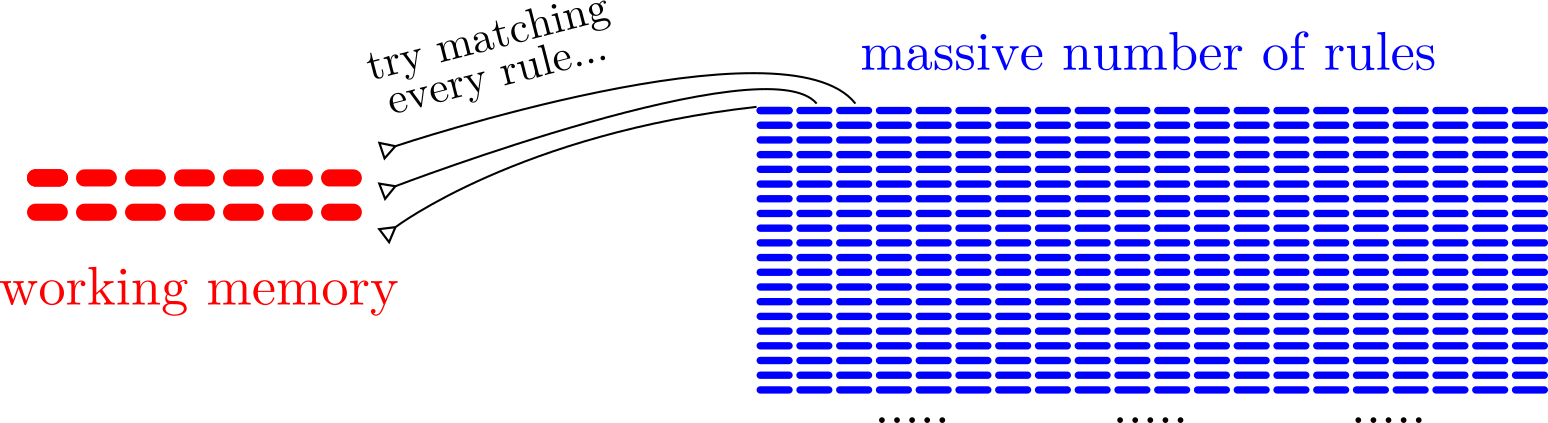
\includegraphics[scale=0.8]{rete-explained-1.png}}}
\end{equation}
Instead, the \textbf{Rete algorithm} compiles the rules into a \textbf{classification tree}, so that each new Working Memory item is matched by ``filtering'' through the tree:
\begin{equation}
\vcenter{\hbox{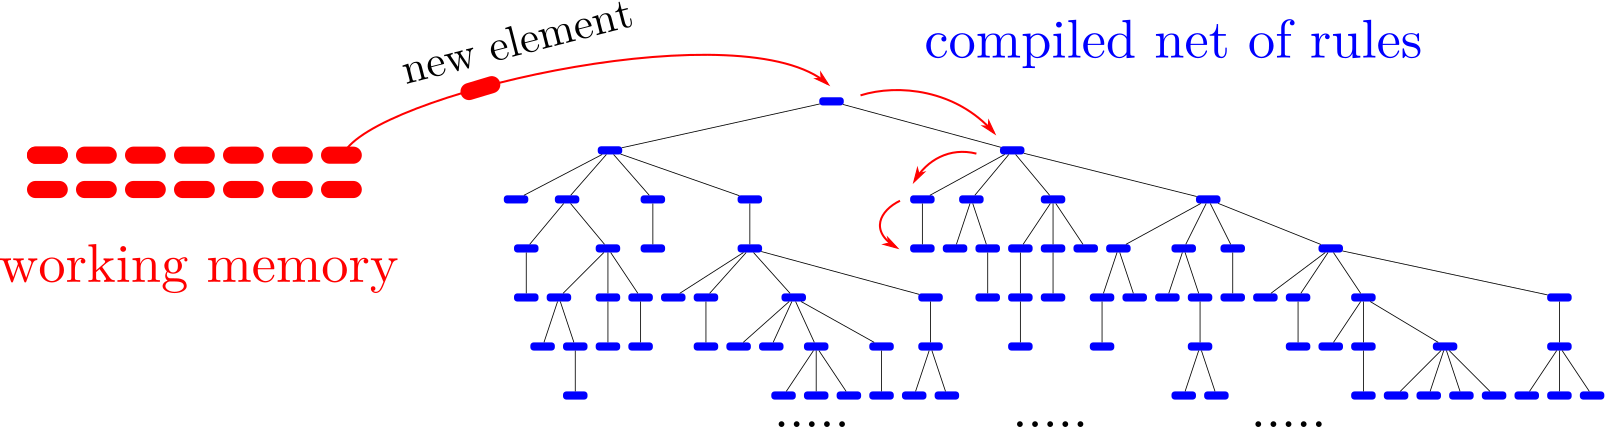
\includegraphics[scale=0.8]{rete-explained-2.png}}}
\end{equation}

So how does the Transformer perform rules matching?  It seems that rules are stored in the $Q, K, V$ matrices.  The Self-Attention mechanism is like a \textbf{message-passing} algorithm that yields a logic rule as its result:
\begin{equation}
\vcenter{\hbox{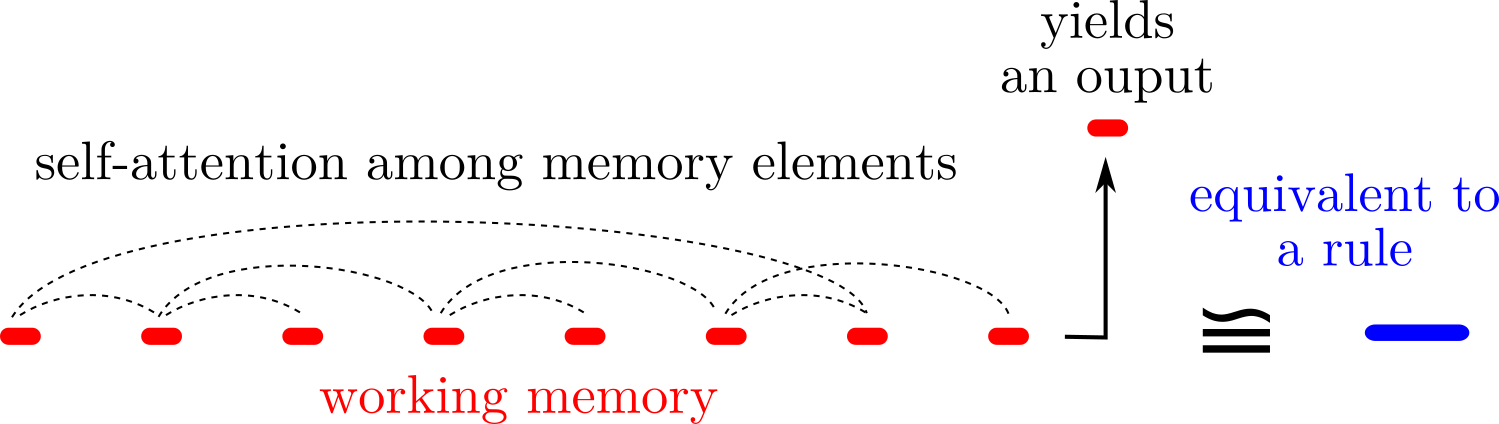
\includegraphics[scale=0.8]{rete-explained-3.png}}}
\end{equation}

\end{document}
